%% This file is based on Michael Shell's
%% bare_conf.tex
%% V1.4b
%% 2015/08/26
%% by Michael Shell
%% See:
%% http://www.michaelshell.org/
%% for current contact information.
%%
%% This is a skeleton file demonstrating the use of IEEEtran.cls
%% (requires IEEEtran.cls version 1.8b or later) with an IEEE
%% conference paper.
%%
%% Support sites:
%% http://www.michaelshell.org/tex/ieeetran/
%% http://www.ctan.org/pkg/ieeetran
%% and
%% http://www.ieee.org/

%%*************************************************************************
%% Legal Notice:
%% This code is offered as-is without any warranty either expressed or
%% implied; without even the implied warranty of MERCHANTABILITY or
%% FITNESS FOR A PARTICULAR PURPOSE! 
%% User assumes all risk.
%% In no event shall the IEEE or any contributor to this code be liable for
%% any damages or losses, including, but not limited to, incidental,
%% consequential, or any other damages, resulting from the use or misuse
%% of any information contained here.
%%
%% All comments are the opinions of their respective authors and are not
%% necessarily endorsed by the IEEE.
%%
%% This work is distributed under the LaTeX Project Public License (LPPL)
%% ( http://www.latex-project.org/ ) version 1.3, and may be freely used,
%% distributed and modified. A copy of the LPPL, version 1.3, is included
%% in the base LaTeX documentation of all distributions of LaTeX released
%% 2003/12/01 or later.
%% Retain all contribution notices and credits.
%% ** Modified files should be clearly indicated as such, including  **
%% ** renaming them and changing author support contact information. **
%%*************************************************************************

\documentclass[conference]{IEEEtran}
\usepackage[utf8]{inputenc}
\usepackage{cite}
\usepackage{graphicx}
\usepackage{url}
\usepackage{color}
%\usepackage{hyperref}
\usepackage{flushend}

\usepackage{glossaries}
\loadglsentries{acronyms}

\newcommand{\cappos}[1]{\textcolor{red}{[Justin: #1]}}

\definecolor{dkgreen}{rgb}{0,0.60,0}
\newcommand{\albert}[1]{\textcolor{dkgreen}{[Albert: #1]}}
\newcommand{\lukas}[1]{\textcolor{blue}{[Lukas: #1]}}


% correct bad hyphenation here
\hyphenation{op-tical net-works semi-conduc-tor}


\begin{document}

\title{Practical Fog Computing With Seattle}


% author names and affiliations
% use a multiple column layout for up to three different
% affiliations
\author{\IEEEauthorblockN{Albert Rafetseder}
\IEEEauthorblockA{NYU Tandon School of Engineering\\
albert.rafetseder@univie.ac.at}
\and
\IEEEauthorblockN{Lukas Pühringer}
\IEEEauthorblockA{NYU Tandon School of Engineering\\
lukas.puehringer@nyu.edu}
\and
\IEEEauthorblockN{Justin Cappos}
\IEEEauthorblockA{NYU Tandon School of Engineering\\
jcappos@nyu.edu}}

% make the title area
\maketitle

%!TEX root = paper.tex
\begin{abstract}

In this paper we present Seattle, a practical and publicly accessible
platform with considerable deployment history.
Seattle's sandbox implementation solves the widely-recognized issue
of node heterogeneity in \gls{fc}, and 


het = [nodes, networks, ops]

and deployment models.
Seattle's Python-based sandbox runs on multiple
operating systems and platforms.
Our system architecture supports heterogeneous
deployment models, from isolated/standalone and peer-to-peer to
full-fledged provisioning by a dedicated operator.

\albert{Mention the term ``federation''.}

% This characteristic, while taken
%for granted in Internet services, but often overlooked in the context
%of \gls{fc}.
Seattle's components and interfaces are
designed for compatibility and reuse, and align with the trust boundaries
that exist between different stakeholders.

Besides our own use of Seattle as a distributed network testbed for
teaching and research, outside groups have used existing Seattle
components, and constructed new components with compatible interfaces,
to adapt the platform to their needs. This has resulted in edge node
selection tools based on social graphs, an Android-compatible computing
sandbox that can access smartphone sensors, \albert{etc.}

\lukas{Maybe be more explicit about how Seattle solves ALL fog issues? \\
Edge location (NAT): tcp relay \\
heterogeneity: Mac/Linux/Windows/Routers (OpenWRT)/ Raspberries (Raspbian)/ Android \\
mobility/number of nodes/geographical distribution: clearinghouse, advertiseserver \\
privacy/security: sandboxing \\
interoperability/federation: modular architecture \\
sensor networks: seattle spinoff/Sensibility \\
}

Seattle is FOSS, .... ?

\end{abstract}

%!TEX root = paper.tex
\section{Introduction And Related Work}

In recent years, \gls{fc} has established itself as an approach to
cloud computing at the edge of the network. Fog systems are typically
characterized by the large number of geographically distributed
nodes, ranging
from embedded systems, like network connected
sensors, to smartphones and end-user laptops
\cite{Bonomi:2012:FCR:2342509.2342513,Yi:2015:SFC:2757384.2757397,dastjerdi_fog_2016}.
While leveraging the
ubiquitous availability and specific capabilities of such devices brings
many opportunities, it also carries new challenges unknown to traditional cloud
services. Such challenges include the heterogeneity of fog
nodes~\cite{Bonomi:2012:FCR:2342509.2342513,7868354,Yi:2015:SFC:2757384.2757397,mahmud_fog_2016},
their accessibility, e.g. behind private networks, and extended security and
privacy requirements \cite{botta_integration_2016}.

Another issue is that existing proposed \gls{fc} architectures have
been described
as ``siloed''~\cite{belli_design_2015}, referring to the lack of
open interfaces that characterize today's fog devices and infrastructures.
Furthermore, opportunities and challenges have been widely addressed in the
respective literature from a theoretical point of view, but actual \gls{fc}
implementations --- let alone actively deployed and
publicly available platforms that can be used in fog contexts --- are rare.

In this paper, we introduce our Seattle platform and make the case for
why its unique design is well suited for \gls{fc} applications. But,
to provide context, we first review relevant aspects of the existing
literature.

\subsection{Related Work}

Emerging technologies have opened potentially promising new areas for research
in \gls{fc}. Bellavista et al.~\cite{bellavista_feasibility_2017} investigate the
applicability of Docker containers for \gls{fc}. The work uses and extends
the open-source Kura framework to create \gls{IoT} gateways that control information
flow between fog nodes and the cloud, while also reviewing and benchmarking
different container-related technologies used in these nodes.
The focus of this work is on \gls{IoT} computing, where tailored services run
on fog nodes to gather data that is forwarded to the cloud for further processing.
A similar evaluation of Docker containers for edge computing can be found in
\cite{ismail_evaluation_2015}.

Others have contributed fog platforms for very specific use cases, e.g.
an emergency alert system using smartphones that propagate alerts to nearby
emergency departments \cite{7134091}, an idea also proposed by Masip-Bruin
et al.~\cite{masip-bruin_foggy_2016}. Gazis et al. introduce an ``Adaptive
Operations Platform''
to effectively apply equipment failure models to the fog computing
infrastructure of Industrial
\gls{IoT} \cite{gazis_components_2015}.
Amrutur et al.\cite{amrutur_open_2017} discuss the use of
a testbed for "smart city" apps that could be mounted on
light poles. Vehicular use cases, including ones that are based on
ad-hoc networks, are presented by Bitam et al.~\cite{bitam_vanet-cloud:_2015}
and Truong et al.\cite{truong_software_2015}.

Apart from individual use cases, some implementations address specific individual
\gls{fc} issues, like Dsouza et al. who propose a policy management framework
to authenticate the various actors in applications
like smart transportation systems \cite{dsouza_policy-driven_2014}.
Yi et al.~\cite{yi_fog_2015} points out vendor lock-in
as a possible problem for \gls{fc}, and attempts to exploit locality
in a real-world experiment with face recognition software.

In addition to academic work, commercial business solutions using fog computing
have also evolved.
Cisco IOx~\cite{cisco_iox} promotes a
system that allows traditional Linux application development on
Cisco IOS powered networking devices.
Google recently released ``Google \gls{IoT} cloud,'' a system for
cloud based device management and a protocol bridge to connect edge nodes to
cloud analytic systems~\cite{google_iot_core} and other infrastructure.

Finally, there are different stances on operational aspects of
\gls{fc} platforms. Some authors assume a centrally-managed and
operated approach, perhaps including monetarization~\cite{mahmud_fog_2016,7868354}, whereas others~\cite{belli_design_2015}
call for open interfaces and interoperability so that many
fog environments can coexist and provide federated services.

As will be discussed shortly, our platform Seattle offers a practical,
useable sandbox implementation that tackles the widely-acknowledged
node heterogeneity issue in \gls{fc}. Furthermore, Seattle's components
are designed for loose coupling and precise trust boundaries, so as to
enable multi-stakeholder operations. This enables out-of-the-box
deployments with minimal mutual trust requirements.
All the Seattle components described in this paper are active, live, and
publicly accessible. All software is
\acrlong{FOSS}, and available from public
repositories\footnote{\texttt{\url{https://github.com/SeattleTestbed}}}.


\subsection{Contributions}

The contributions of this paper are as follows:
\begin{itemize}
\item We present Seattle, a platform uniquely adaptable for
 \gls{fc} research and applications. Seattle is
capable of real-world deployment on heterogeneous nodes,
including desktop and laptop machines, Android devices,
Raspberry Pis,
and routers and embedded devices running OpenWrt.
%Seattle nodes host Python-based \glspl{VM} that can run
%general-purpose code on a variety of platforms,
%and which self-isolate so as to not
%affect the safety and performance of the host node.
\item We explain how
Seattle's system architecture can cater to a variety of use cases,
ranging from peer-to-peer deployments to full-fledged
provisioning by a dedicated operator, to cooperative setups,
where different stakeholders federate and unite multiple parallel running
instances of services.
\item We present our live deployment of Seattle which has been
installed on tens of thousands of devices, and used by over 4,000
researchers and students during its 8 years of operational history.
\end{itemize}
Our past deployments of Seattle have served multiple contexts
including research~\cite{li2015fence,rafetseder2013sensorium,zhuang2014sensibility,Eisl1010:Service,Tuts1010:Sustained,collares2011smart,zhuang2015privacy,cappos2014blursense,7133607} and education~\cite{Wallace_CCSC_2011,Cappos_CCSCCP_2010,Cappos_CCSCNW_2009,Cappos_SIGCSE_2014,Hooshangi_SIGCSE_2015}.
In addition, other groups have successfully reused and augmented Seattle components
for their own specific purposes~\cite{chard2010social,chard12ssc,caton2014social,muller2014tomato,tomato,eittenberger2012doubtless,zhuang2012distributed,zhuang2014taking,tredger2013building}.
 % which includes related work
%!TEX root = paper.tex
\section{System Architecture}

We discuss in this section the governing principles behind Seattle's
segmentation of functionality into self-sufficient yet interoperable
components.
An important insight for Seattle as a platform is how the classical
dichotomy of platform operators and users gives way to multi-faceted
trust relationships between a large number of mutually-unrelated
stakeholders.
In Seattle, the actual edge-based software installs, core infrastructure
services, clearinghouse operations, platform software builds, and remote
application deployments might be carried out and managed by different
groups of people, potentially untrusted (or even unknown) between groups
and among members of the same group.
% Then why/how do people trust each other in such a system?


\subsection{Goals And Design Principles}

From the above we can see that the system architecture must be able
to keep the needs of the various parties apart. To facilitate this,
components are designed along these trust boundaries.

Not all components are strictly required for Seattle's functioning.



\albert{...for breaking things into interoperable components. These are a subset of foggish goals (which might include performance isolation etc.)}


\albert{Roughly: 1, separate along trust boundaries. 2, make parts self-sustainable and useful by themselves. 3, stable inter-component interfaces. 4, flexible UIs.}


\subsection{Components}
\albert{These guys implement additional foggish goals.}


%!TEX root = paper.tex
\section{Implementation}

\subsection{In-House Implementations}

Talk about how the sandbox achieves foggish goals: portability, isolation.

Mention device manager and practical problems like NAT.

Mention the clearinghouse because we have other clearinghouses
to talk about later.

\subsection{Community Contributions}


\section{Practical Deployment}\label{sec-deployment}

As mentioned previously, we have running implementations of all
Seattle components on nodes on the public Internet, including
many instances we neither control or operate. These latter
implementations have been contributed to our Clearinghouse's
resource pool by volunteers.
Apart from the numbers we report below, we do not have any
insight on offspring projects that reuse our open-source software
base, but set up their own independent deployments. Seattle has
no tracking code besides what an operating Clearinghouse
needs to support the sandboxes it controls.

To assess the current scale and size of Seattle, we report
statistics from \gls{IP} addresses contacting our Software
Updater service. This service is contacted
by all installations to which Seattle's main Installer Builder
has shipped end-user devices, and has reported downloads from more
than 40,000 different \gls{IP} addresses during our eight years
of deployment history.
This metric is not perfect: it undercounts multiple devices behind
a \gls{NAT} gateway, and overcounts devices that change their
\gls{IP} address frequently (such as mobile nodes). However, it
gives an impression of the scale of our deployment.

Attempting to reverse-resolve these \gls{IP} addresses to \gls{DNS}
names yields no result for about 50\% of the responses; of the
remainder, 30\% belong to home Internet providers; and 15\% to
university machines (which likely includes students since they
spend time on the campus). Note also that the number of online
nodes (and thus sandboxes) varies over time, as device owners
turn off or suspend their devices as they move, or as their daily
routines start and end.
Figure~\ref{fig:map} plots a world map of Seattle nodes, with the
colors encoding the approximate node density in an area.
The node locations were generated from GeoIP data.
It shows that Seattle has notable user bases outside of the
United States (where its development originally started),
particularly in Central Europe and China.

Since its inception,
more than 4,000 experimenters have used Seattle's Clearinghouse
to request access to resources on remote devices. We attribute this
to the fact that our Clearinghouse offers ten free sandboxes for
every registered user, and contributing one's own resources counts
as a ``credit'' to use more remote sandboxes in turn.
Resource credits have proven a valuable incentivation strategy
to push the adoption of Seattle.

While offering generous resources to bootstrap experiments,
Seattle has also benefitted greatly from generous contributions
of code, documentation, tutorials, and libraries from more than 100
contributors at 32 institutions all over the world.
Seattle strives to make contributing easy. All of its components
are open-source software, and thus easy to inspect, adapt, and
reuse in other contexts.

Sensibility Testbed~\cite{zhuang2014sensibility} has been particularly
successful in adapting and reusing Seattle components. It extends
Seattle's sandbox type so as to allow access
to sensors on Android smartphones and tablets. Furthermore, its
Device Manager includes an additional \gls{GUI} in the form of
a native Android app. Sensibility Testbed's Clearinghouse implements
special policies not found in Seattle. An experimenter requesting
sandboxes on Sensibility must first complete
an \gls{IRB} approval process, which ensures that the experiment
conducted does not impact the privacy of device owners involved.


\begin{figure}
  \centering
  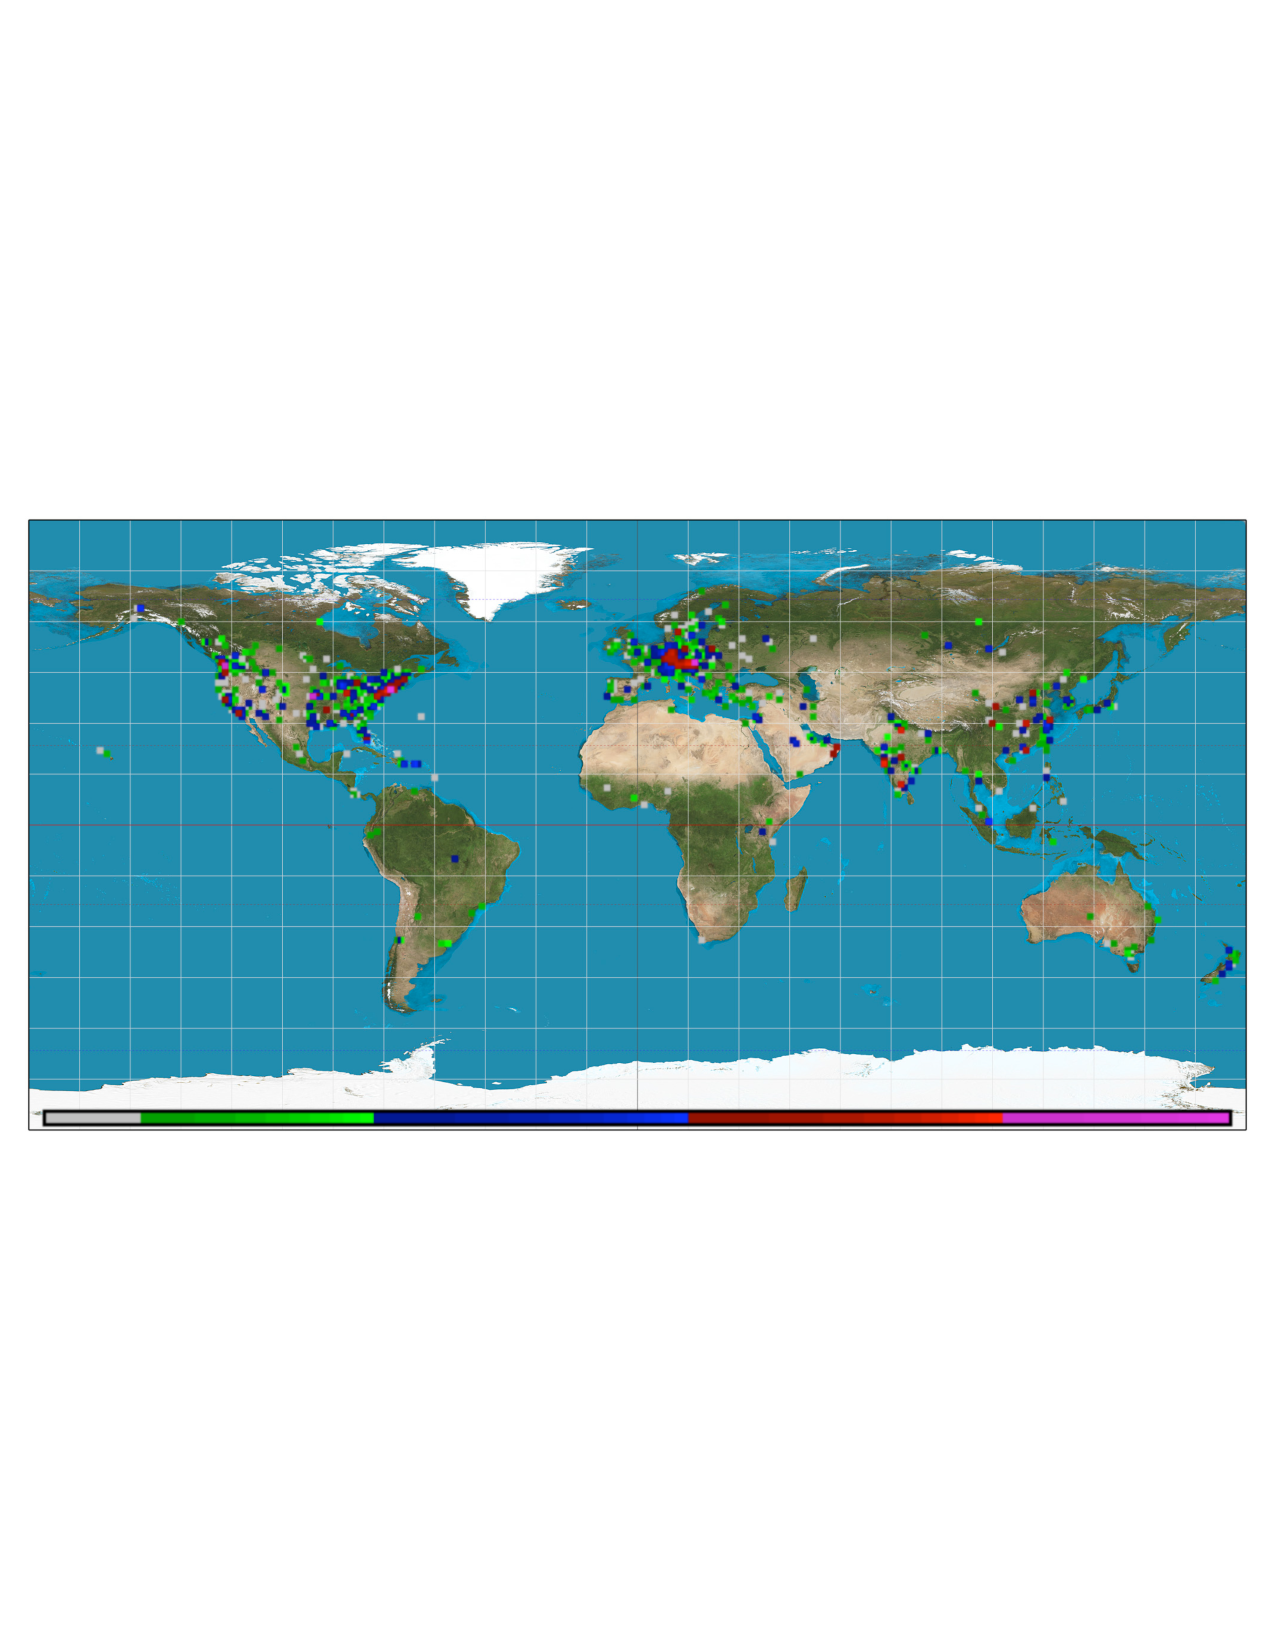
\includegraphics[width=\columnwidth]{figures/finishedmap_ipinfo_small.pdf}
  \caption{World map of Seattle node locations. Color shows approximate density from low (grey) to high (magenta).}
  \label{fig:map}
\end{figure}

%!TEX root = paper.tex
\section{Conclusion And Outlook}

This paper presents Seattle, a practical and publicly accessible
platform for \gls{fc}. Seattle is deployed and operational in the
real world on heterogeneous nodes,
including desktop and laptop machines, Android devices,
Raspberry Pis,
and routers and embedded devices running OpenWrt.
Seattle's installer packages and sandbox implementation
thus address a widely-recognized and central issue for the
success of \gls{fc}, node heterogeneity.

The system architecture of Seattle consists of loosely-coupled
components. This makes the components useful as stand-alone entities,
and stimulates reuse and adaptation of existing component
implementations for unforeseen purposes.
Furthermore, since components are separated along trust boundaries,
%different implementations of many components (such as the sandbox
%or the Clearinghouse) exist. All implementations can coexist and
Seattle does not require a single centralized operator for all
components. Instead, a large range of operational scenarios with
varying scopes can be implemented: from fully locally setups to
peer-to-peer resource swapping and federated multi-operator
deployments with mutually-trusted intermediaries.
Seattle's support of heterogeneous operations includes and exceeds
the capabilities of often-assumed centrally managed and
operated \gls{fc} setups.

We have an active, live, and publicly accessible deployment of all
Seattle components described in this paper.
More than 4,000 experimenters have used our existing deployment
to run distributed experiments; over 100 developers from 32 institutions
have contributed to Seattle's free, open-source software stack since
its inception in 2009.
Seattle has been installed on 40,000 devices all over the world, and
has been used
for teaching and research; outside groups have used existing Seattle
components, and constructed new components with compatible interfaces,
to adapt the platform to their needs.
All of Seattle's software is \acrlong{FOSS} and available on GitHub.


\bibliography{references,seattle_us,seattle_them}
\bibliographystyle{plain}

\end{document}


